\RequirePackage{ifpdf}
\documentclass[a4paper,11pt]{kth-mag}

\usepackage[T1]{fontenc}
\usepackage{textcomp}
\usepackage{lmodern}
\usepackage[latin1]{inputenc}
\usepackage[swedish,english]{babel}
\usepackage{modifications}

%Egna paket

%For graphics
\usepackage{graphicx}
\usepackage[section]{placeins}%Makes floats stay in place
\usepackage{caption}
\usepackage{subcaption}
\captionsetup{compatibility=false} %Problem with subcaption workaround

\usepackage{gensymb} % Provides \degree \textdegree


%Egna kommandon
%\let\oldsection\section
%\renewcommand{\section}[1]{
%\FloatBarrier
%\oldsection{#1}
%\FloatBarrier
%}




\title{Efficient features for representing hand shape in images}

\subtitle{Using a classeme-based approach}

\foreigntitle{Effektiva visuella formdeskriptorer för handigenkänning}
\author{Patrik Berggren}
\date{Juni 2014}
\blurb{Master's Thesis at NADA\\Supervisor: Hedvig Kjellström\\Examiner: Danica Kragic}
\trita{TRITA xxx yyyy-nn}
\begin{document}
\frontmatter
\pagestyle{empty}
\removepagenumbers
\maketitle
\selectlanguage{english}


%Acknowledgements
%Hedvig såklart för handledning, ideer, kritik, kommentarer
%Akshaya hjälp med att sätta upp systemet, hans master uppsats, references

\begin{abstract}
%TODO
Abstract to come
\end{abstract}
\clearpage
\begin{foreignabstract}{swedish}
%TODO
Abstract to come
\end{foreignabstract}
\clearpage
\tableofcontents*
\mainmatter
\pagestyle{newchap}

\chapter{Background}
\section{Introduction}
Today, there is a shift in the ways we interact with computers taking place.
Previously, it has mainly been through keyboards and mouse, but today you find that there are touchscreens, wii, kinect and speech-recognition.
Even though the applications are still limited, there have also been some research into hand pose estimation (HPE), meaning to estimate the hand gesture or hand pose that the user does.
This has proved difficult, but have some important applications.
It is of course very useful for recognizing sign language, but other applications include learning from demonstration,
%TODO fler applikationer 

However, hand pose estimation is difficult and is generally considered that we have still to find a good approach for it.
There are many problems involved with hand pose estimation which will be discussed later.
One of the biggest challenges is that the hand can move in many different ways i.e. have many degrees of freedom, which makes hand tracking difficult.
This is also a strongly contributing fact to the discontinuity between the image and the hand pose.
Furthermore, this mapping is a many-to-many mapping which further complicates the problem.
The goal of this thesis is, nevertheless, to overcome these problems to some degree and to hopefully contribute with a new way of doing HPE.

The basis of this thesis is an earlier master thesis done by Akshaya Sridatta Thippur %Citera kolla namn
in which he investigated which image features was most suitable for HPE.
This thesis will expand that idea and continue from the image feature that was judged to have the overall best properties, which was HOG features (%Referera till section).
 

\section{Modelling the hand}
\subsection{Hand anatomy}
It is important to understand the hand anatomy as that must be the basis to construct a modell.
Understanding the underlying anatomy gives a clue of which aspects that are important to capture in our modell.
On one hand a too simple hand modell will result in an unnatural modell where a lot of possible hand motions are impossible in the modell.
However, one doesn't want a too complex modell either since that will make hand pose estimation harder.
Before we discuss the actuall hand model we should take a short look at the hand anatomy to understand the choice of model better.

Figure~\ref{fig:hand} shows a X-ray of a human hand which normally have 27 bones. 
%TODO Marieb, Elaine N (2004). Human Anatomy & Physiology (Sixth ed.). Pearson PLC. ISBN 0-321-20413-1.
The bones at the base of the palm is called Carpals from which the base of the fingers strectch out.
Each finger consists of bone parts starting from the base, metacarbals, proximal phalanges, intermediate phalanges, and distal phalanges, except from the thumb which doesn't have the intermediate phalange.

\begin{figure}[!ht]
    \centering
    \begin{subfigure}[t]{0.35\textwidth}
        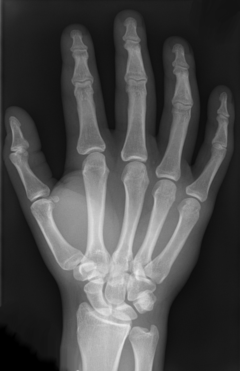
\includegraphics[width=\textwidth]{images/handskeletone.png}
        \caption{X-ray of a human hand}
        \label{fig:hand}
    \end{subfigure}
    \begin{subfigure}[t]{0.55\textwidth}
        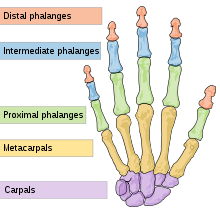
\includegraphics[width=\textwidth]{images/labeledhand.png}
        \caption{A hand with labeled bones}
        \label{fig:hand}
    \end{subfigure}
\end{figure}

One might be surprised at the many bones in the hand, but what is really  of interest to us is what degrees of freedom exists.
That is, in how many different ways can we move the hand.
It is here neccessary to destinguish between two different kinds of freedom.
Firstly have the DOFs (degree of freedom) that the hand can move in on itself.
However, we also have DOFs which the hand physically be put into, but is not capable of doing on its own.
For instance, each finger can be slightly rotated if a torque is put on it, but there is no muscle that can perform this motion.
Apart from that, we must also consider that many DOFs are restricted in their range.
There is for instance a limit to how far back one can pull the fingers before they break.
As if all this is not enough we can as Akshaya points out include a lot of other things in our model such as skin-color, subject-specific joint constraints, and hand size.
The conclusion is that some simplifications must be done to obtain a workable hand model.

\subsection{Hand modell}
%Distinktion mellan hand pose och hand pose model är inte så viktig eftersom att de korresponderar med varandra. En linjär ändring i den ena innebär i stort en linjär ändring i den andra.
The first simplification that we will do is to neglect all aspects of the hand that is not related to how the actual hand pose, that is the joint angles.
However, after that we are still left with a few choices to make if we doesn't want to model all possible DOFs of all joints.
%TODO beskriv vilken hand modell som det blir 


A common range for dimensionality of a hand pose is 30-50 degrees %Akshaya master
although there are exceptions.
If the aim is to reduce dimensionality, one can for instance try to form constraints on the dy
Furthermore, as noted in
%Full DOF
one might model the hand with some constraints.

\section{Hand pose estimation}
%Schematisk bild över stegen
When it comes to hand pose estimation it can't be said that there is a widely accepted correct way of doing things.
Instead, there is many different approaches to HPE.
Firstly, we should distunguish between quite different settings under which HPE could be done.
The easiest and most successfull approach is to use a glove with sensors or markings from which it is easy to collect data of how the hand is moving.
The problem with such approaches is that a glove or other sensor that needs to be put on the hand is intrusive and hinders the user from moving the hand freely.
Furthermore, it normally requires callibration and will generally be less accessible to the user.
Therefore, there have been research to estimate a hand pose from one or multiple cameras.
Using multiple cameras allow for additional information to be used and one can for instance estimate depth and to some degree remove the difficulty that self-occlusion and ambuigity otherwise causes.
However, this thesis is about estimating hand pose from a single camera.
This is a reasonable setting especially if we consider a robot learning a task from demonstration.
In that case it is unlikely that two cameras on the robot will provide much new information since they will normally have to be quite close to each other and one therefore opts for a single camera instead.
Using a single camera also makes the technology more accessible to more applications in general.


\subsection{HOG features}
When doing HPE and image recognition in general one normally doesn't work directly with the pixels of the image.
Instead, one extract what is called image features from the image that in some sense are meant to either capture some semantic meaning of the image or at least some feature that is less local than a single pixel.
Some of the features that are regurarly used in HPE is Histogram of Oriented Gradients (HOG)\cite{HOG}, silhouette-based features, Scale-invariant feature transform (SIFT),  Hu-moments, Shape Context Descriptors and others.  

The idea of HOG is that images can be described by the intensity gradients that it contains.
That is, the directions in which the intensity increases the most in different parts of the image.
The first step in computing a HOG feature is dividing the image into cells, which is normally just a rectangular grid over the image, but could be done in other ways.
The gradients is then computed in each cell and the distribution is recorded in a histogram.
It is common to ignore orientation of the gradient so that opposite pointing gradients are put into the same bin, but here again it is possible to use bins from 0 to $360\degree$.
To make the features more robust from illumination differences the feature values are extracted from blocks of several cells where the intensity gradients have been normalized.

Originally, the HOG features where used to detect humans in images\cite{HOG}, but have since then been used in other applications including hand pose estimation. 
%Några HOG referenser
As can be seen in figure~\ref{fig:HOG_girl} the histograms can be said to roughly keep information about the edges in the image. 

\begin{figure}
    \centering
    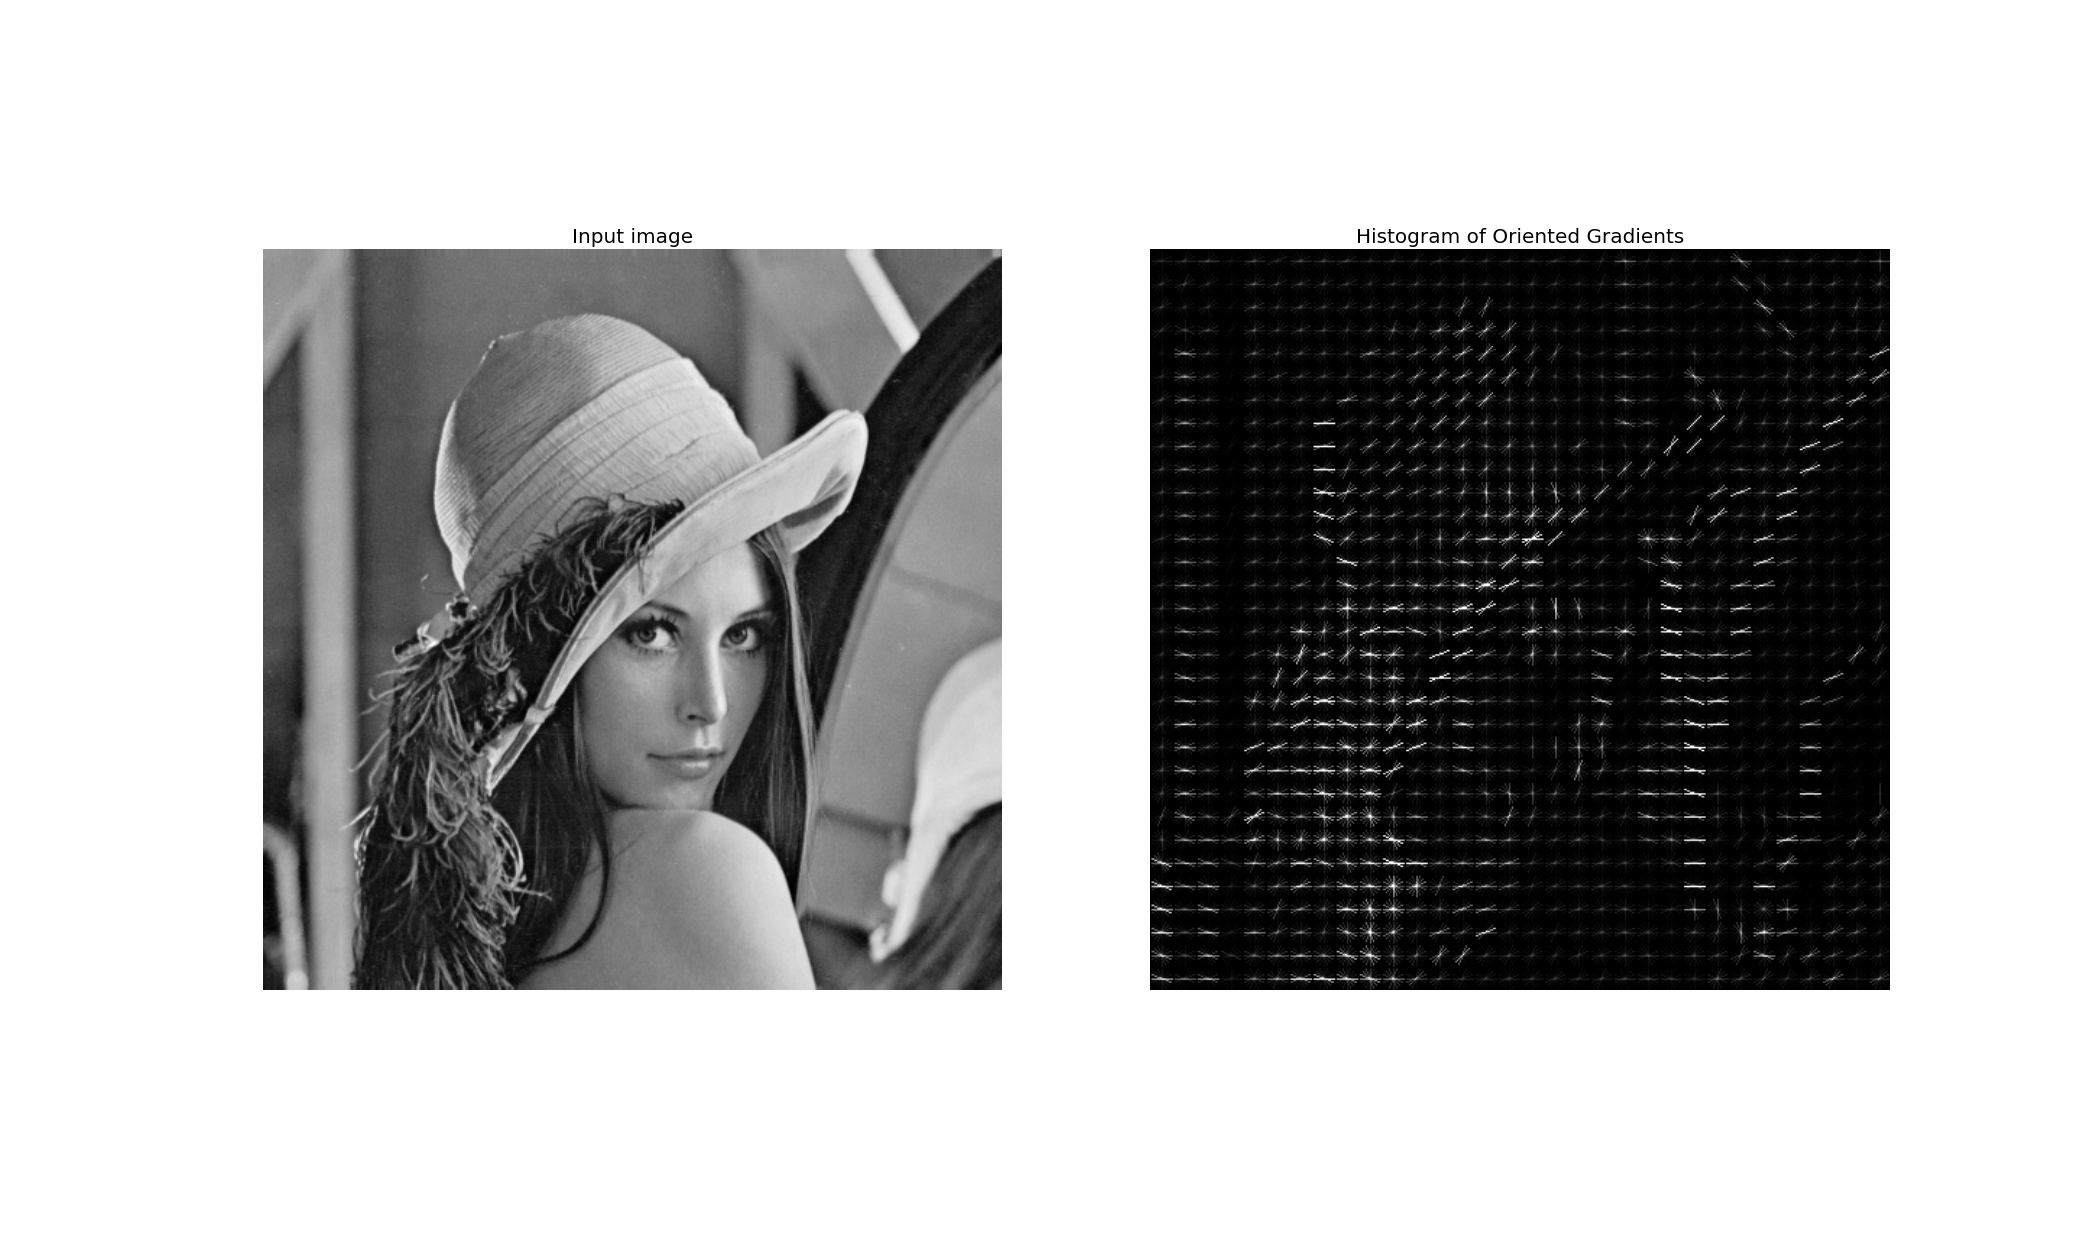
\includegraphics[width=\textwidth]{images/hog_lena_old.png}
    \caption{The image to the right shows the corresponding gradients of the cells from the input image (left).} 
    \label{fig:HOG_girl}
\end{figure}


\subsection{Smoothness, generativity and discriminativity}
\label{sec:featureproperties}
When evaluating image features we are interested to have the properties smoothness, generativity and discriminativity.
The first, smoothness, simply says that we would like for a small change in feature values to correspond to a small change in hand pose parameters.
This is as Akshaya notices far from the case for most image features.
In his results he tests linear transitions between hand poses which correspond to linear transitions in hand pose parameters (i.e. joint angles).
Ideally, the features would then change close to linearly as well and it is this property that we will call smoothness.
The reason we would like smooth image features is because they would be better suited for regression.
The other two aspects that we are interested in is concerned with what sort of mapping we have from features to hand pose.
We would like to have a one-to-one mapping, but that is generally not possible and so we must relax that requirement and say that we want something as close as possible to a one-to-one mapping.
Generativity in this case means that we would like the same hand pose to generate the same image features, or at least to generate image features within a small subspace in the feature space.
To understand this one can consider two images of the exact same hand pose, but under different lightings which would affect many image features to at least some degree.
We are also interested in discriminativity which is concerned with the other direction of the mapping.
That is, how unimodal the inverse mapping is.
Are there many hand poses that generate the same image features? It is for instance probable that figure (TODO två figurer som ger liknande HOGs)
 %todo
%Figure på baksida och framsida av hand
will generate similiar features for any image feature that tries to detect edges.


\subsection{A new descriptors}
%Slutgiltig schematisk bild över tanken
This thesis is about a novel way of getting hand descriptors.
However, before the descriptor is explained in more detail, the research from which this idea stems from must be explained.

\subsubsection{Classemes}
In a quite recent paper (2010) a new approach for object category regocnition was proposed\cite{classeme1}.
That is, given an image the classifier should classify the image as either belonging to or not belonging to a specific category.
The problem with many earlier approaches is that the classifiers doesn't scale well, and that learning new categories is very expensive or in fact impossible without relearning the whole classifier\cite{classeme1}.

The idea is to use a predetermined set of classifiers that one can combine to learn new categories.
The predetermined classifiers are learned by doing an web image search for a specific term to collect positive examples for that term, however, no human cleanup is used and so certain images might be rather unexpected.
If we now want to learn the new category duck we might be interested in what the classifiers for water and bird gives as output.
However, this is not entirely correct as the original classifiers are not supposed to have a semantic meaning, but rather use ancillary image characteristics.
For instance, a bird classifier might look for a V shaped object for the beak.
The authors points out that it is those ancillary image characteristics that is probably useful when combined and as can be seen in their results some of the new categories uses object classes that certainly doesn't seem to have any semantic connection\cite{classeme1}.

More specifically, when a new category is learned and when positive examples for that category is gathered one runs each of the original classifiers.
From those one obtains a binary vector where each element corresponds to the output of the corresponding classifier.
This vector is termed the descriptor vector and is all that is used when learning the new category.
It should be noted that to learn the original classifier a more advanced, namely $LP-\beta$, classifier is trained, but as noted in the paper those are trained prior to learning any novel categories and so it isn't of much importance if the orignal classifiers are computationally expensiv.

There have been subsequent papers on this idea, see \cite{classeme2,classeme3}.
They largerly use the same method, but with some modifications.
For instance, in \cite{classeme3} the classemes are learned as meta-classes meaning that they doesn't even have an apparant semantic meaning as in \cite{classeme1,classeme2}.

\subsection{A new descriptor}
This thesis introduces a novel descriptor that is loosely based on the idea of classemes from the previous section. 
However, the connection is somewhat vague as we first of all have a regression rather than classification problem.
The idea is however still to use multiple regressors instead of classifemes.
Assuming that a set of regressors has been choosen the goal would be that we could perform a regression to obtain a mapping from the descriptors to the pose space.
The quality of the reggresion function depends on how well suited the descriptor is in regard to smoothness, generativity and discriminativity as discussed in section~\ref{sec:featureproperties}.

So, how is these regressors formed.
This thesis will investigate if projections onto lines in the HOG space can serve as regressors.
However, it is far from obvious how these lines should be choosen.
Some of the questions one might ask are summarized below.
\begin{itemize}
\item
Should the lines be created from points close together in the HOG space and is there any requirement on the corresponding points in the pose space?
\item
Can we evaluate an individual line to tell if it is likely to be of use without using the whole descriptor?
\item
Should we only use two points for each line or can we use more than two? Might we in fact draw lines that doesn't go through any of the training points?
\item
It seems likely that a line that is far from a point doesn't help a lot in the prediction and so if possible it would likely be useful to weight which lines are used for the prediction.
\end{itemize}
These are some of the questions that will be investigated in this thesis and the experiments carried out are descriped in more detail in the section TODO %TODO metoddel

\bibliography{references}{}
\bibliographystyle{plain}

\appendix
%\addappheadtotoc

\end{document}
